\subsection{Direct Pickup by Bolometers/Sensors}

\paragraph{Description:}
Most CMB experiments use single-moded beam-forming elements to couple bolometers and free-space photon modes in the telescope. In AdvACT, spline-profiled feedhorns [Simon SPIE] \cite{Simon} define the EM mode exciting the orthomode transducer; in POLARBEAR-1 and Simons Array, silicon lenslets excite a planar sinuous antenna. In both cases, imperfect coupling (i.e. reflections) between beam-forming elements and the superconducting antennae can allow ``direct'' coupling between trapped microwave photons and the bolometers. The interaction of trapped light and the bolometer structures (considered as absorbers) is not the subject of this investigation. We assume thermal excitation of absorbing dielectric elements can produce excess microwave power in these devices.

\paragraph{Plan to model and/or measure:}
In principle, we are concerned with mistaking direct-absorbed signal for signal from the pixel microwave lines. As a proxy, we choose to investigate bolometers which we believe have weak or non-existent coupling to these lines due to fabrication or handling (called direct coupling-only devices), and compare the variation of bias powers with atmospheric loading for these bolometers and others. Direct coupling-only detectors are put forward based on initial visual inspection of the detector wafers used in AdvACT arrays. However, the visual assay cannot confirm that any particular bolometer in the array will or will not see the sky through pixel coupling. 

Aside from these possibly sky-insensitive devices, we have known devices which do not couple to the sky and are not near a horn aperture (dark detectors) and the many bolometers which do respond to the sky as intended (pixel-coupled detectors). We use precipitable water vapor (PWV) divided by sin(altitude) as a proxy for atmopsheric loading.

With the AdvACT high-frequency array field data from 2017, we find that some of the potential direct coupling-only (all solid lines) actually behave much like optical devices as seen in Fig. \ref{direct_pickup_PA4}. However, others follow the trend of the intended dark devices (dashed lines in the same figure), and we can compare these devices more directly to the dark bolometer response.

\begin{figure}[h!]
\centering
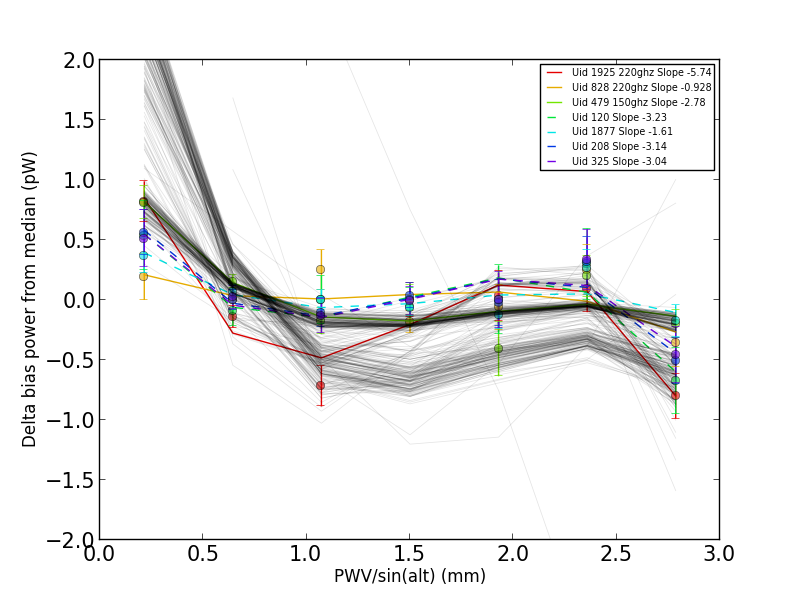
\includegraphics[width=0.8\textwidth]{figures/pickup_test.png}
\caption{Trends vs. atmospheric loading of detector bias power. Solid black lines are pixel-coupled, dashed lines are intentionally dark, and solid colored lines are direct coupling-only candidates.}
\label{direct_pickup_PA4}
\end{figure}

In the end, we do not expect this result to form a strong systematic over overestimating in-band signal based on direct heating of the bolometer. We can perform a null test on flat-field correction or microwvae efficiency to see if weakly-coupled bolometers suffer from non-sky signal pickup differently than well-coupled devices. The specific direct coupling-only candidates will likely not be run through this analysis.

\paragraph{Uncertainty/Range:}
Unfortunately this method doesn't directly compare time-domain signal size between these two classes of bolometers. This can be done once the accidental dark devices have been identified, which we have done for PA4 from the data in the figure. On the other hand, low statistics (few detectors present at a feedhorn exit aperture without being connected to the microwave circuitry of the pixel) make this a challenging effect to consider across the entire array. We do not have any reason to assume other detectors in other parts of the array should behave differently, but we cannot yet compare these numbers to expectations for other bolometers/designs.

\paragraph{Parameterization:}
A figure of merit could be the best-fit scaling of the trends of bias power vs. atmospheric loading for pixel-coupled and the direct coupling-only devices. The baseline to this measurement would be the average best-fit scaling between true dark and pixel-coupled bolometers.
